\cleardoublepage
\chapter{外文翻译}
\section{原文出处:}
\subsection*{题目:\\Physics-informed graph neural Galerkin networks: A unifiedframework for solving PDE-governed forward and inverse problems}
\subsection*{作者:Han Gao, Matthew J. Zahr, Jian-Xun Wang}
\subsection*{期刊名:Computer methods in applied mechanics and engineering}
\newpage

\section{摘要}
尽管物理知情神经网络(PINN)在解决正问题和逆问题方面有着巨大的前景,但是一些技术挑战成为更复杂和更现实的应用的障碍。
首先,大多数现有的 PINN 都是基于全连接网络来学习连续函数,这些函数具有较差的可扩展性和硬边界强制性。
其次,无穷搜索空间使网络训练的非凸优化过于复杂。
第三,尽管基于卷积神经网络(CNN)的离散学习可以显著提高训练效率,但是 CNN 难以处理非结构化网格的不规则几何形状。
针对这些问题,提出了一种基于图卷积网络(GCN)和偏微分方程(PDE)变分结构的离散 PINN 框架,用于统一求解正、逆偏微分方程(PDE)。使用分段多项式基可以降低搜索空间的维数,便于训练和收敛。
该方法不需要对经典 PINN 中的惩罚参数进行调整,可以严格施加边界条件,同化正反两种情况下的稀疏数据。
GCNs 的灵活性被用于非结构化网格的不规则几何图形。该方法在线性和非线性偏微分方程控制的各种正向和反向计算力学问题上显现出优势。
\section{介绍}
偏微分方程(PDE)在工程应用中占有重要地位,因为控制自然或人为复杂系统的大多数物理问题都是由偏微分方程描述的。
然而,寻找解决大多数偏微分方程是一个具有挑战性的问题,这可能涉及复杂的数值技术和可能是耗时的,特别是在参数或初始/边界条件部分已知的情况下。
最近,物理信息神经网络(PINN)[1]作为求解正向和逆向偏微分方程的一种新范式,由于其与传统的数值方法相比具有很大的灵活性和简单性而受到越来越多的关注。
PINN的主要想法是用深度神经网络来逼近PDE的解,手段主要通过结合PDE残差和数据偏差的损失函数。这种独特的损失函数使得物理信息的训练得到提升,不仅结合了PDE本身还有稀疏的数据。

对于如何建立PDE残差项的神经微分算子,PINN可以被分为两类方法:连续和离散。连续的PINNs通常采用全链接神经网络来逼近关于时空坐标$(x,t)$连续的解函数$f(x,t)$,其中关于空间和时间的导数项计算基于自动微分算法。
由于Raissi 等人[1]关于连续 FC-PINN 解决正向和反向偏微分方程惊艳的贡献,连续 PINN 正在经历一个复兴。
它的优点和有效性已经在许多领域的大量科学应用中得到证明[3-7]。例如,在流体应用中,PINN 已经被用于在没有训练标签的前向参数设置中的理想化血管流动问题的快速替代建模[8]。
此外,PINN 也已经在逆向建模设置中制定,以从心血管问题中的可观察数据(例如浓度数据)中提取不可观察的信息(例如血流速度)[9-12]。
Jin 等[13]应用 FC-PINN 求解从层流到湍流的 Navier-Stokes 方程,而 Mao 等[14]进一步证明了它们在高速流动问题上的有效性。
最近,NVIDIA 开发了一个基于连续 PINN 的可扩展实现 SimNet,并将其应用于解决具有大规模 GPU 并行化的各种多物理问题[15]。

尽管由于其巨大的灵活性而取得了巨大的成功和快速的发展,但是目前连续的 PINN 仍然存在一些局限性。
首先,它们受到高训练成本的影响,因为在高维时空(和参数)域中的大量配置点上的点式制定需要大量的 AD 计算[16,17]。
其次,对于连续的 PINN,制定严格的初始/边界条件(IC/BC)是具有挑战性的,这在寻找正确的单一PDE的解方面是有效的,特别是当标记数据非常稀缺甚至不存在时[8]。
尽管可以引入基于距离的特定解决方案,使用专门设计的代数表达式或低容量神经网络[8,18] ,在几个简单的2-D 域上严格施加 IC/BC,但是它未能显示对于真实世界应用的复杂几何形状的有效性。


为了降低训练成本,提高学习效率,利用卷积运算和数值离散化的离散 PINN 已经开始激发兴趣,因为它们具有更好的效率和可伸缩性[19,20]。
具体而言,在离散 PINN 中常用卷积神经网络(CNN)来直接学习整个时空解场的端到端,并且基于数值离散代替逐点 AD 计算物理信息损失的所有导数项。
例如,Zhu 等[19]开发了一种物理约束的卷积编码器-解码器来解决高维椭圆偏微分方程,而 Geneva 等[21]进一步将该框架扩展到具有参数初始条件的动态双曲偏微分方程。Zhang 等[22]提出了一个物理指导的 CNN 用于地震响应建模,也探索了类似的想法与一个递归神经网络(RNN)用于非线性结构的元建模[23]。
Wandel 等[24]最近提出了一种参数设置下基于自回归 U 网的无数据流体替代方法。在上述工作中,计算区域是正则的,离散化的统一网格,其中偏微分方程残差计算的差分(FD)方法。这是因为基于 FD 的神经网络基本上植根于矩形区域的结构化笛卡尔网格。
除了基于 FD 的 PINN 之外,有限体积(FV)离散化也被用来构造基于 PDE 的损失函数来解决稳态流体问题,然而,由于经典卷积运算的固有局限性,这仍然限于矩形域[25]。为了使基于物理知识的 CNN 能够用非结构化网格解决不规则域上的参数偏微分方程,Gao 等[20]提出了一种基于几何自适应物理知识的 CNN,PhyGeoNet,其将预先计算的坐标映射嵌入到经典的 CNN 结构中。
尽管 PhyGeoNet 的有效性已经在简单的不规则域上得到了证明,但是对于一般的复杂几何形状来说,它仍然具有挑战性。

针对目前存在的问题,我们提出了一种基于广义卷积运算的非结构化网格的新的离散化PINN框架来处理不规则域。也就是说,卷积操作直接对非结构化网格数据进行,这些数据可以看作是离散的非欧几里德流形,即图。
此外,PDE信息图卷积网络(GCN)结构的构造受到有限元(FE)方法的启发[26,27] ,这是另一种经典的数值离散技术,对于物理知情学习具有许多优点。
首先,由于偏微分方程残差的变分形式(弱形式) ,其中 Neumann 边界条件可以自然地包含在控制方程的弱形式中,微分算子的阶可以通过部分积分有效地降低,从而大大降低了学习的复杂性。
此外,强形式 PINN 所需要的大量搭配点可以是被相对较少的正交点所取代,这可能潜在地减少相当大的训练成本。对于连续型 PINN,变分(弱)形式最近得到了发展,并且已经显示出对于强形式 PINN 的显著优越性。

在这些变分连续的 PINN 中,通常建立一个逐点全连通的神经网络,结合多项式测试函数,以 Petrov-Galerkin 的方式制定变分形式。
由于深层神经网络具有黑盒特性,精确的正交法则难以建立,这导致与变分形式相关的额外误差。此外,基本边界条件不能以硬约束的方式加入。
Yao 等[34]提出的 FEM-Net 是一个基于 FE 的离散 PINN,其中基于 FE 的卷积已被开发用于为 CNN 构建变分偏微分方程残差。
然而,这种方法是在线性假设下,并且经典的CNN仍然受限于矩形区域。

本文提出了一种基于图卷积网络和偏微分方程变分结构的离散 PINN 框架,用于统一求解正、逆偏微分方程。具体而言,新的贡献概述如下:

(a)将图卷积运算引入物理信息学习中,充分利用基于有限元的离散化方法对非结构化网格的不规则域进行离散化。
与基于经典 CNN 的离散 PINN 不同,该方法不需要网格化,因为它可以像传统的有限元求解器那样直接处理带有单纯形/四边形单元的非结构网格。

(b)采用一组有限维多项式基函数重建基于 Galerkin 公式输出节点解图的全场预测,从而大大缩小搜索空间,方便训练。此外,由于两个测试/试验函数都基于标准多项式,变分积分可以用高斯求积精确计算。

(c)所建议的 PINN 设计能够准确地满足必要的边界条件,避免了在大多数 PINN 中使用BC 软约束执行来调整惩罚系数。

(d)提出一项新的数据同化方案,以严格执行观测数据。

\section{方法}
\subsection{概述}
考虑一个在有界区域$\Omega\subset R^d$的物理系统,由一组非线性,稳定的参数化偏微分方程以通用的离散形式控制,
$$R(U(\mu);\mu)=0$$
其中$\mu\in R^{N_\mu}$为PDE的参数向量,$U:R^{N_\mu}\rightarrow R^{N_U}$为离散化参数相关的解,$R:R^{U}\times R^{N_\mu}\rightarrow R^{U}$代表离散PDE算子。
偏微分方程组受边界条件(BC)的约束,边界条件定义在区域的边界条件$\partial \Omega$ 上。

在这项工作中,我们针对这种偏微分方程控制系统在正向和逆向问题,提出了一个创新的物理知情图神经伽辽金网络(PI-GGN)以建立一个解决方法。
在正问题中,我们的目标是得到给定已知边界条件和参数$\mu$的解 U;对于反问题而言,当系统的 BC 和参数$\mu$部分已知时,并且有状态的稀疏观测,从而对问题进行求解。
在所提出的框架中,设计了一个 GCN 来学习一组非结构化网格上的状态节点解。基于连续伽辽金方法重构了物理损失函数中的偏微分方程残差项。
系统的基本边界条件以硬约束的形式加入,附加的数据可以被同化来同时求解正问题和逆问题。该方法的每个部分都将会在以下小节中详细说明。
\subsection{对非结构化数据的图神经网络}
由于 GCN 在处理非结构化数据方面具有极大的灵活性,人们对将其应用于科学机器学习问题越来越有兴趣。通过经典的数据驱动,基于图表的学习在模拟各种计算力学问题方面表现出色[35-40]。
通常,通过定义非欧几里德空间的卷积运算,GCNs 将 CNN 类型的结构推广到图形数据。对图的节点之间的依赖关系进行建模的能力是使 GCNs 能够处理有任意边界的非结构化网格数据。
从图1可以看出,一个图由节点和边构成,其中每个节点都是由自身的特征向量$f$定义,而节点之间的关系就用边来描述。一个节点的邻接集$N(\cdot)$指的是和该节点通过边相连的所有节点集合。
因此,一个具有非结构化网格和对应节点处的解的网格能够自然的被图自然的定义出来。和基于CNN的离散PINN类似,GCN也用来解决离散的解$U(\bar{\mu})\approx \hat{U}(\Theta^*)$,其中$\Theta^*$是 GCN 对于$\bar{\mu}$的训练参数。

\paragraph*{注意:}由于深层神经网络的通用逼近能力,一般情况下,GCN 的输入特征向量可以由网格离散成任意空间变化的域。
在这项工作中,GCN 接受一个输入图,其中每个节点与其网格的空间坐标相关联,然后将离散解域作为输出图输出,其中每个节点包含相应的节点解向量


和CNN类似,输出的解可以通过在输入层的多次图卷积操作得到,通过消息传递函数逐次更新节点信息。可以写成
$$\boldsymbol{f}_{i}^{(l)}=\gamma^{(l)}\left(\boldsymbol{f}_{i}^{(l-1)}, \square_{j \in \mathcal{N}(i)}^{(l)} \Psi^{(l)}\left(\boldsymbol{f}_{i}^{(l-1)}, \boldsymbol{f}_{j}^{(l-1)}\right)\right),$$
其中i记为第i个节点,$l$记为第$l$层$\gamma\Psi$为非线性可微函数,$\square$记为可微置换不变函数(例如,求和、平均值或最大值)。
特征向量可以由$\boldsymbol{f}_{i}^{(l)} \in \mathbb{R}^{N} \boldsymbol{f}^{(l)} $和$ \boldsymbol{f}_{i}^{(l-1)} \in \mathbb{R}^{N} \boldsymbol{f}^{(l-1)}$其中$ N_{\boldsymbol{f}^{(l-1)}}$和$ N_{\boldsymbol{f}^{(l)}}$分别为第(l-1)和l层特征维度。

为了实现的简单性,所有的节点特性通常都被连接起来,变成一个更大的向量 X。边缘连接的信息存储在一个稀疏矩阵 A 中,称为邻接矩阵。
在实际应用中,边缘被用来隐含地表达邻接矩阵。在这项工作中,GCN 是基于 Chebyshev 谱图卷积算子[41]构建的,该算子源于谱卷积定理[42] ,其中引入了切比雪夫多项式以避免昂贵的特征分解。
具体来说,Chebyshev 图卷积的消息传递函数可以写成:
$$\boldsymbol{X}^{l}=\operatorname{ReLU}\left(\sum_{k=1}^{K} \boldsymbol{Z}^{(l-1, k)} \cdot \boldsymbol{\Theta}^{(I-1, k)}+\boldsymbol{b}^{l-1}\right)$$

其中$\Theta^{(l-1, k)}$为第(l-1)层第k个基底的可训练参数,$\boldsymbol{b}^{(l-1)}$为偏置值向量,第k个基递归计算方式如下:

$$\begin{array}{l}
    \boldsymbol{Z}^{(l-1,1)}=\boldsymbol{X}^{(l-1)} \\
    \boldsymbol{Z}^{(l-1,2)}=\hat{\boldsymbol{L}} \cdot \boldsymbol{X}^{(l-1)}, \\
    \boldsymbol{Z}^{(l-1, k)}=2 \hat{\boldsymbol{L}} \cdot \boldsymbol{Z}^{(l-1, k-1)}-\boldsymbol{Z}^{(l-1, k-2)},\\
    \hat{\boldsymbol{L}}=\boldsymbol{L}-\boldsymbol{I}\\
    \boldsymbol{L}=\boldsymbol{I}-\boldsymbol{D}^{-\frac{1}{2}}A\boldsymbol{D}^{\frac{1}{2}}
    \end{array}$$
在这里$K$设为10.

\subsection{变分形式的物理信息损失项}
损失函数通常基于PDE残差项,稳定场景的PDE可以写成:
$$(6)\nabla \cdot F(u, \nabla u ; \boldsymbol{\mu})=S(u, \nabla u ; \boldsymbol{\mu}) \text { in } \Omega$$
其中$u: \Omega \rightarrow \mathbb{R}^{N_{c}}$为解,$F: \mathbb{R}^{N_{c}} \rightarrow \mathbb{R}^{N_{c} \times d}$为流函数,
$S: \mathbb{R}^{N_{c}} \rightarrow \mathbb{R}^{N_{c}}$为源项,$\nabla:=\left(\partial_{x_{1}}, \ldots, \partial_{x_{d}}\right)$记为在区域中的微分算子。
因此上式可以代表很大一部分静态偏微分方程,如泊松方程、线性弹性方程和纳维尔-斯托克斯方程等。

\subsubsection{弱形式的PDE残差项}
对于连续的FC-PINNs来说,计算损失项中的微分是通过自动微分在逐点处计算的,并且FCNN 作为连续试探函数搜索无穷维解空间。
因此,无限搜索空间使网络训练的非凸优化过于复杂,通常需要大量的配置点。在这项工作中,我们使用分段多项式基,以减少搜索空间的维数,并促进物理知识的训练/收敛。
具体来说,守恒定律(Eq。(6)采用节点连续伽辽金方法离散,用连续分段多项式基函数构造试验空间
$$\mathcal{V}_{h}^{p}=\left\{v \in\left[\mathcal{H}^{1}(\Omega)\right]^{N_{c}}|v|_{K} \in\left[\mathcal{P}_{p}(K)\right]^{N_{c}}, \forall K \in \mathcal{E}_{h}\right\}$$

其中 $\mathcal{H}^{1}(\Omega)$ 为Sobolev空间, $\mathcal{P}_{p}(K)$ 为定义在单位元K上次数至多为p的多项式空间, $\mathcal{E}_{h}$为有限元网格。
测试空间和$\mathcal{V}_{h}^{p}$相同且解$u_{h} \in \mathcal{V}_{h}^{p}$对任意测试函数$ \omega_{h} \in \mathcal{V}_{h}^{p}$满足PDE的弱解形式,

$$\int_{\partial \Omega} \omega_{h} \cdot F\left(u_{h}, \nabla u_{h} ; \boldsymbol{\mu}\right) n d S-\int_{\Omega} \nabla \omega_{h}: F\left(u_{h}, \nabla u_{h} ; \boldsymbol{\mu}\right) d V=\int_{\Omega} \omega_{h} \cdot S\left(u_{h}, \nabla u_{h} ; \boldsymbol{\mu}\right) d V .$$

我们引入 $\mathcal{V}_{h}^{p} $的基函数 $\boldsymbol{\Phi}(x) \in \mathbb{R}^{N_{\boldsymbol{U}} \times N_{c}}$  来表示测试变量 $\omega_{h}(x)=\boldsymbol{\Phi}(x)^{T} \tilde{\boldsymbol{W}}$, 
其中 $\tilde{\boldsymbol{W}} \in \mathbb{R}^{N_{\boldsymbol{U}}}$  为基函数中变量系数, 利用测试函数系数的任意性可以形成Galerkin形式的等价形式:

$$\int_{\partial \Omega} \boldsymbol{\Phi} \cdot F\left(u_{h}, \nabla u_{h} ; \boldsymbol{\mu}\right) n d S-\int_{\Omega} \nabla \boldsymbol{\Phi}: F\left(u_{h}, \nabla u_{h} ; \boldsymbol{\mu}\right) d V-\int_{\Omega} \boldsymbol{\Phi} \cdot S\left(u_{h}, \nabla u_{h} ; \boldsymbol{\mu}\right) d V=0 .$$

我们引入$\{(\beta^v_i,\tilde{x}_i^v)\}^{N_{qv}}_{i=1},\{(\beta^s_i,\tilde{x}_i^s)\}^{N_{qs}}_{i=1}$分别作为在$\Omega,\partial \Omega$上积分的权重和点,并且定义残差为:

$$(10)\begin{aligned}
    \boldsymbol{R}(\tilde{\boldsymbol{U}} ; \boldsymbol{\mu})= & \sum_{i=1}^{N_{q s}} \beta_{i}^{s} \boldsymbol{\Phi}\left(\tilde{x}_{i}^{s}\right) \cdot F\left(\tilde{u}_{h}\left(\tilde{x}_{i}^{s} ; \tilde{\boldsymbol{U}}\right), \nabla \tilde{u}_{h}\left(\tilde{x}_{i}^{s} ; \tilde{\boldsymbol{U}}\right) ; \boldsymbol{\mu}\right) n- \\
    & \sum_{i=1}^{N_{q v}} \beta_{i}^{v} \nabla \boldsymbol{\Phi}\left(\tilde{x}_{i}^{v}\right): F\left(\tilde{u}_{h}\left(\tilde{x}_{i}^{v} ; \tilde{\boldsymbol{U}}\right), \nabla \tilde{u}_{h}\left(\tilde{x}_{i}^{v} ; \tilde{\boldsymbol{U}}\right) ; \boldsymbol{\mu}\right)- \\
    & \sum^{N_{q v}} \beta_{i}^{v} \boldsymbol{\Phi}\left(\tilde{x}_{i}^{v}\right) \cdot S\left(\tilde{u}_{h}\left(\tilde{x}_{i}^{v} ; \tilde{\boldsymbol{U}}\right), \nabla \tilde{u}_{h}\left(\tilde{x}_{i}^{v} ; \tilde{\boldsymbol{U}}\right) ; \boldsymbol{\mu}\right),
\end{aligned}$$
其中$\tilde{u}_h:\Omega\times R^{N_U}\rightarrow R^{N_c}$为在$V_h^p$上离散状态向量的连续表示,即:
$$\tilde{u}_h(x;\tilde{U})=\Phi(x)^T\tilde{U}$$
表面和体积积分系数($\beta^s$ 和 $\beta^v$)存储为常数张量,在网络训练过程中保持不变。基函数 $\Phi$ 的矩阵是在有限个求积点上得到的,可以预先计算为常张量$(\Phi(\tilde{x}^v), \Phi(\tilde{x}^s),\nabla\Phi(\tilde{x}^v),\nabla\Phi (\tilde(x)^s))$。
给出了偏微分方程残差(Eq(10))将用于定义 GCN 的物理信息损失函数。即 GCN 学习节点解向量 U 作为输出图 $U(\theta)$ ,它以坐标$(X)$作为输入图。当偏微分方程参数 $\mu$未知时,它们可以作为可训练的参数,与网络参数 $\theta$ 一起更新。流量函数和源函数$(F,S)$都是可微函数,梯度信息可以从输出传播到输入。表1总结了这些注释。

\subsubsection{必要的边界约束}
我们通过限制无约束自由度,即原理必要的BC来施加约束:
$$\boldsymbol{R}_u(\boldsymbol{U}_u(\mu),U_e;\mu)=0$$
其中$U_e$为BC上已知值,$U_u(\mu)$为无约束自由度$\boldsymbol{U}(\boldsymbol{\mu})$对应的序号。
在神经网络设置中,我们通过将自由度划分为无约束(未知)和约束(已知)自由度$\hat{\boldsymbol{U}}(\Theta)=(\hat{\boldsymbol{U_u}}(\Theta)^T,\hat{\boldsymbol{U}}_c^T)^T$来强制执行边界条件。
并使用基本 BC (即$ \boldsymbol{U}_c = \boldsymbol{U}_e$)的已知值来定义约束自由度;通过最小化物理信息损失函数定义无约束自由度,损失函数可以写为:
$$\mathcal{L}_{\mathrm{f}}(\boldsymbol{\Theta} ; \boldsymbol{\mu})=\left\|\boldsymbol{R}_{u}\left(\hat{\boldsymbol{U}}_{u}(\boldsymbol{\Theta}), \boldsymbol{U}_{\boldsymbol{e}} ; \boldsymbol{\mu}\right)\right\|_{2} .$$

在该公式中,基本边界条件将通过构造自动满足,这与连续FC-PINN形成鲜明对比,连续FC-PNN将FCNN定义为逐点解函数,这对硬边界执行提出了挑战.

\subsection{统一正反问题}
GCN 可以基于 Eq13 中定义的物理信息损失函数进行训练。解决下列无监督优化:
$$\Theta^{*}=\underset{\Theta}{\arg \min } \mathcal{L}_{\mathrm{f}}(\boldsymbol{\Theta} ; \overline{\boldsymbol{\mu}}),$$
其中 $\Theta^{*}$表示最优网络参数,$\mu$表示已知的偏微分方程参数,然后用 GCN 求解正向偏微分方程(正向解)。然而,在许多情况下,一些物理参数如材料性质、入口速度和雷诺数等是不可用的,相反我们可以获得稀疏的观测数据(标签)$U_o$,这些数据可以同化来推断未知参数(反解)。
在先前的 PINN 方法中,解决反问题以一种软约束的方式同化数据 $U_o$ 来求解,其中物理损失被数据损失分量增加。也就是说,我们可以得到下面的优化公式:
$$\left(\Theta^{*}, \boldsymbol{\mu}^{*}\right)=\underset{\Theta, \mu}{\arg \min } \mathcal{L}_{\mathrm{f}}(\boldsymbol{\Theta} ; \boldsymbol{\mu})+\lambda \underbrace{\left\|\mathcal{F}^{s 2 o}(\hat{\boldsymbol{U}}(\boldsymbol{\Theta}))-\boldsymbol{U}_{o}\right\|_{2}}_{\text {data loss: } \mathcal{L}^{d}},$$
其中$\mathcal{F}^{s 2 o}$代表从状态到可观测的映射,$\lambda$为惩罚因子。适当地调整惩罚权重$\lambda$对于收敛是至关重要的,然而,这是具有挑战性的,并且经常以实证的方式进行[16]。
在这里,我们介绍了一种新的方法,同化观测数据和推断未知参数,而不需要超参数调整。具体来说,观测数据是通过将 GCN 输出构造为
$$\mathcal{F}^{s 2 o}(\hat{\boldsymbol{U}}(\boldsymbol{\Theta}))=\boldsymbol{U}_{o}$$
因此,通过求解以下约束条件,可以同时得到未知参数$\mu$和边界条件 $\hat(\boldsymbol{U})_u$ 以及偏微分方程解:
$$\left(\Theta^{*}, \boldsymbol{\mu}^{*}\right)=\underset{\Theta, \boldsymbol{\mu}}{\arg \min } \mathcal{L}_{\mathrm{f}}(\boldsymbol{\Theta} ; \boldsymbol{\mu}), \quad \text { subject to: } \quad \mathcal{F}^{s 2 o}(\hat{\boldsymbol{U}}(\boldsymbol{\Theta}))=\boldsymbol{U}_{o} .$$

\paragraph*{算法}:\\
\begin{algorithm}
\caption{算法1 通过GCN解决PDE正问题} 
\KwIn{PDE参数$\bar{\mu}$,点集坐标$X$和邻接矩阵$A$}
\KwOut{解$\hat{\boldsymbol{U}}$}
在点集上预计算矩阵基函数$\Phi$得到$ \boldsymbol{\Phi}\left(\tilde{x}^{v}\right), \boldsymbol{\Phi}\left(\tilde{x}^{s}\right), \nabla \boldsymbol{\Phi}\left(\tilde{x}^{v}\right), \nabla \boldsymbol{\Phi}\left(\tilde{x}^{s}\right)$\\
得到在(10)中定义的残差函数$\boldsymbol{R}(\tilde{\boldsymbol{U}};\boldsymbol{\mu}) $\\
带入计算得到(12)\\
划分自由度$\hat{\boldsymbol{U}}(\boldsymbol{\Theta})=\left(\hat{\boldsymbol{U}}_{u}(\boldsymbol{\Theta})^{T}, \hat{\boldsymbol{U}}_{c}^{T}\right)^{T}$;强化边界条件$\hat{\boldsymbol{U}}_{c}=\boldsymbol{U}_{e}$;
形成含有物理信息的损失函数;\\
求解(14)中的优化问题来得到$\hat{\boldsymbol{U}}=\left(\hat{\boldsymbol{U}}_{u}\left(\boldsymbol{\Theta}^{*}\right)^{T}, \boldsymbol{U}_{e}^{T}\right)^{T};$
\end{algorithm}

\begin{algorithm}
    \caption{算法2 通过GCN解决PDE反问题} 
    \KwIn{稀疏的观测数据$\boldsymbol{U}_o$,点集坐标$X$和邻接矩阵$A$}
    \KwOut{解$\hat{\boldsymbol{U}}$和PDE中参数$\mu$}
    在点集上预计算矩阵基函数$\Phi$得到$ \boldsymbol{\Phi}\left(\tilde{x}^{v}\right), \boldsymbol{\Phi}\left(\tilde{x}^{s}\right), \nabla \boldsymbol{\Phi}\left(\tilde{x}^{v}\right), \nabla \boldsymbol{\Phi}\left(\tilde{x}^{s}\right)$\\
    得到在(10)中定义的残差函数$\boldsymbol{R}(\tilde{\boldsymbol{U}};\boldsymbol{\mu}) $\\
    带入计算得到(12)\\
    划分自由度$\hat{\boldsymbol{U}}(\boldsymbol{\Theta})=\left(\hat{\boldsymbol{U}}_{u}(\boldsymbol{\Theta})^{T}, \hat{\boldsymbol{U}}_{c}^{T}\right)^{T}$;强化边界条件$\hat{\boldsymbol{U}}_{c}=\boldsymbol{U}_{e}$;
    严格施加观测数据(16),形成含有物理信息的损失函数;\\
    求解(17)中的优化问题来得到$\boldsymbol{\mu}^*$和$\hat{\boldsymbol{U}}=\left(\hat{\boldsymbol{U}}_{u}(\boldsymbol{\Theta})^{T}, \hat{\boldsymbol{U}}_{e}^{T}\right)^{T}$

\end{algorithm}

\section{数值实验}
我们展示了提出的物理知情图伽辽金神经网络(PI-GGN)在各种计算力学问题的正向和反向设置。
具体来说,本文研究了泊松方程、线性弹性方程和具有已知或未知 BCs/参数的 Navier-Stokes 方程,以证明该方法的有效性。
此外,我们还比较了两种不同的同化稀疏观测资料的方法,说明了严格执行参数/场反演资料的优越性。
对于所有情况,GCN 体系结构保持不变,其中隐藏图层中的节点向量的维度固定为[32,64,128,256,128,64,32]。
相对误差度量 e 定义为,
$$e=\frac{\left\|\hat{\boldsymbol{U}}\left(\boldsymbol{\Theta}^{*}\right)-\boldsymbol{U}(\overline{\boldsymbol{\mu}})\right\|_{2}}{\|\boldsymbol{U}(\overline{\boldsymbol{\mu}})\|_{2}},$$
其中 $\Theta^{*}$为计算参数$\bar{\mu} $的训练网络参数。
\subsection{Possion equation}
2DPossion方程
$$\begin{aligned}
    \nabla u + f=0\ in\ \Omega\\
    u=0\ on \ \partial \Omega
\end{aligned}$$
\begin{figure}[H]  
    \centering  
    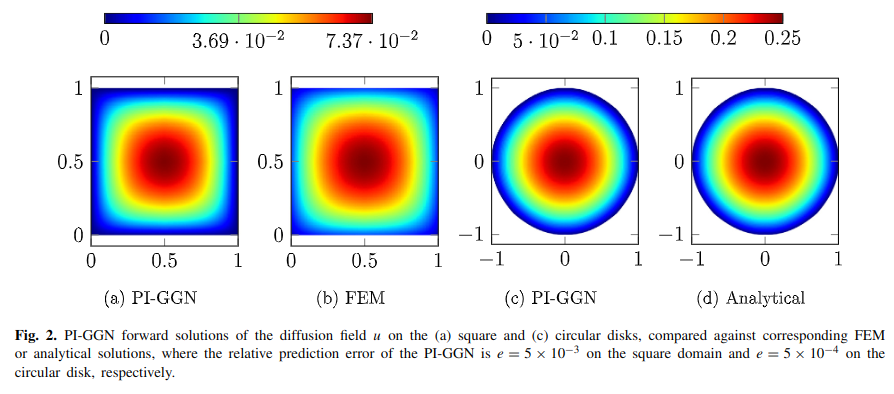
\includegraphics[width=\textwidth]{./pics/Possion.png}  
\end{figure}
\subsubsection{扩散场的正解}
我们首先考虑正向问题,在单位平方域上给出源项 f (f = 1)(图2a 和2b)。
采用四个四边形单元对区域进行离散,并给出了求解和区域变换的三阶多项式基。
结果表明,该图的总节点数为49个,远低于典型的点式 FC-PINN 的配置点总数。PI-GGN 预测的轮廓与有限元参考轮廓非常吻合,相对误差为 $e = 0.5\%$,但在边界附近有误差。

在图2c 中,相同的偏微分方程在一个单位圆形区域上求解,这里存在解析解(图2d)$u(x,y)=\frac{1-x^2-y^2}{4}$。

在 PI-GGN 中,元素个数保持不变,而多项式基的阶被设为两个,因此用25个节点构造图。结果表明,PI-GGN 正演解与解析解基本一致,相对预测误差仅为0.05\% 。
这个简单的测试案例表明,基于图的离散 PINN 可以很容易地处理非结构化网格的非矩形域,这对之前的标准的基于 FD 的 CNN 架构构成了挑战,因为他们需要光栅化或坐标变换等特殊处理[20],使实现和收敛复杂化。
\subsubsection{源项的反问题求解}
其实PI-GGN 的真正强大的作用在于通过同化附加状态观测值同时求解正问题和逆问题。例如,当源项不给定时,PI-GGN 能够同化稀疏数据求解扩散场,同时统一推导未知源项。
这里我们假设常数源项 f = 2是未知的,观察 u 只能在图3a 所示的一个点观察到。我们用两种方法同化数据并解决反问题: 
一种是在(15)中加入一个数据损失作为惩罚项来同化数据,其中超参数选取为 λ = 1000,另一种是严格基于方程(17)的同化。
从图3中我们可以看到他不仅收敛到了真实的源项而且能够正确的模拟出正解,且误差小于1\%。

\subsection{Navier-Stokes 方程}
在最后一个测试样例中,我们研究静态不可压缩NS方程的正反问题,由于他高度非线性的困难,显得非常具有挑战性。定常 NS 方程模拟了具有常密度的粘性流体流动,其表达式为
$$\begin{array}{l}
    (v \cdot \nabla) v-\nu \Delta v+\nabla p=0, \quad \nabla \cdot v=0 \quad \text { in } \Omega, \\
    v=v^{D} \quad \text { on } \partial \Omega^{D} \text {, } \\
    \nu(n \cdot \nabla) v-p n=0 \quad \text { on } \partial \Omega^{N} \text {, } \\
\end{array}$$
其中$v:\Omega\rightarrow \mathbf{R}^d$为速度向量,$p:\Omega\rightarrow \mathbf{R}$为压力,$\nu$为流体的粘度,n为边界上向外的单位法向量。
解向量记为$u=[v_1,v_2,p]$。粘度$\nu$设为0.01。为了稳定性考虑,我们采取了一种混合有限元方法。我们构造了一个单独的子网,用于预测每个解变量 v1、 v2和 p。

\subsubsection{正向模拟解}
首先,我们对一个经典的流动问题——空腔流动进行了测试,该问题定义在一个方形区域上。盖子放在顶部边缘并向右移动$(v_1 = 1, v_2 = 0)$。
其余三个边设置为无滑动边界$(v_1 = v_2 = 0)$。该区域由100个四边形单元离散。速度场和压力场的配置点数分别为441和121。

\begin{figure}[H]  
    \centering  
    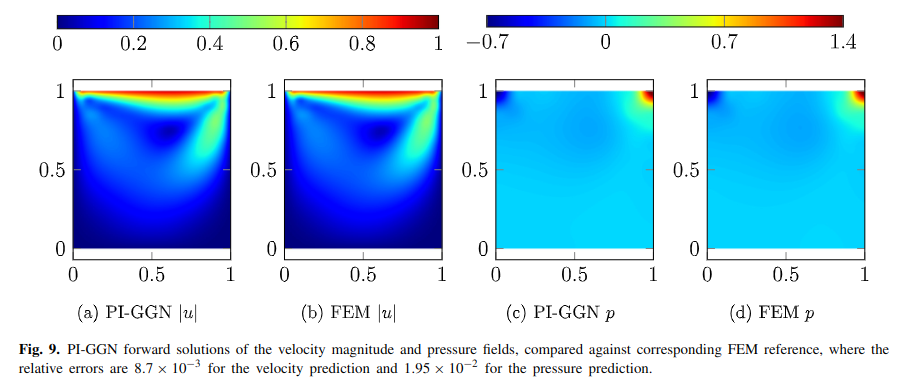
\includegraphics[width=\textwidth]{./pics/p9.png}  
\end{figure}

如图9所示,PI-GGN 的速度和压力正解的轮廓与相应的有限元参考值非常吻合。相对预测误差小于1\% 。
值得注意的是,超过10000个搭配点被用来实现基于 AD 的 FC-PINN 的同等精度水平[16,17]。


\begin{figure}[h]  
    \centering  
    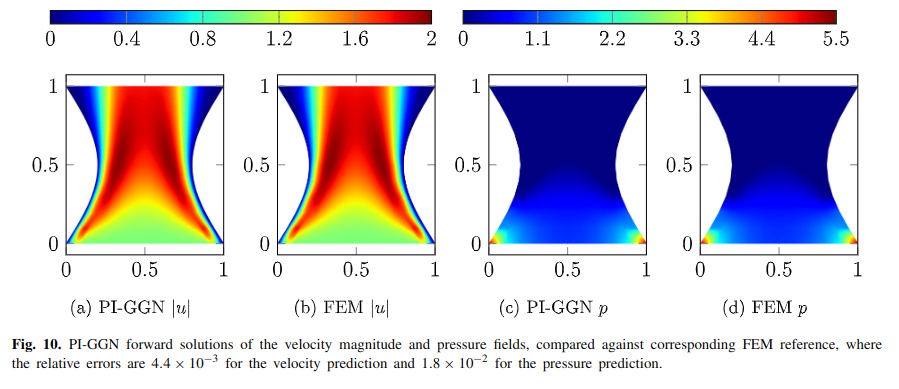
\includegraphics[width=\textwidth]{./pics/p10.png}  
\end{figure}

当然我们还测试了 PI-GGN 在理想狭窄中求解流体流动,其中入口速度设置为底部$(y = 0)的 v^D = [0,1]$,并且在顶部的出口处$(y = 0)$规定了无牵引边界条件。
使用与盖驱动空腔问题相同的有限元设置。类似地,速度场和压力场都可以精确求解,PI-GGN 预测与 FEM 参考结果一致(见图10)

\subsubsection{未知进口速度场和未观测压力场的反问题}

\begin{figure}[h]  
    \centering  
    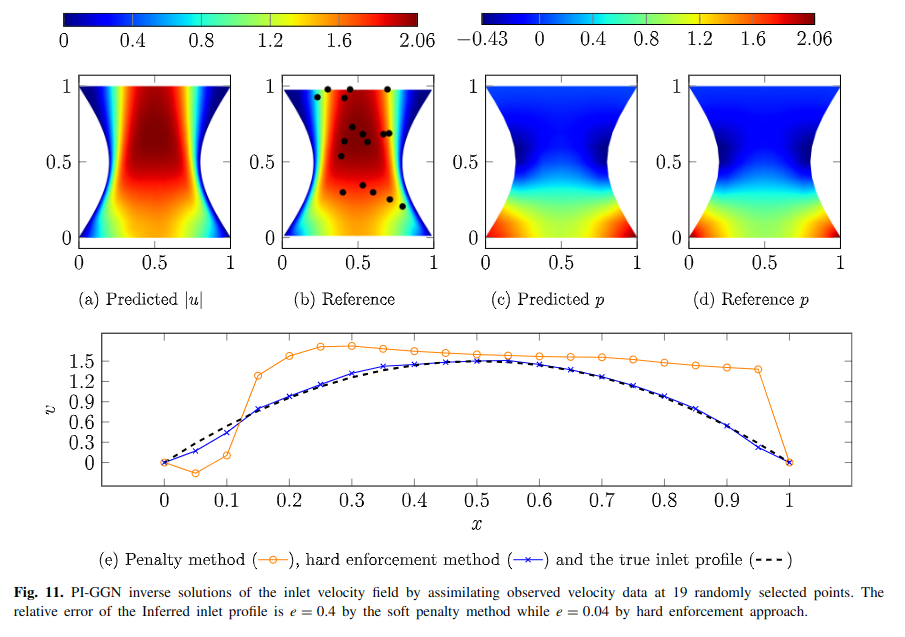
\includegraphics[width=\textwidth]{./pics/p11.png}  
\end{figure}

最后,我们考虑一个由 NS 方程组的反问题。特别是当入口速度场未知时,将通过稀疏速度观测数据来推断,如图11b 所示。
真正的进气道具有如图11e 所示的抛物线形状。剖面的函数形式在求解反问题时没有预先定义。也就是说,反转的尺寸等于进气道的自由度,大于20。
通过对稀疏位置的速度观测数据进行同化处理,该方法能够准确地推断出未知的进气道速度分布,并能很好地恢复整个进气道的速度场和压力场。

然而,我们发现基于惩罚的数据驱动方法推断的进气道并不十分准确,偏离了基本真理。
尽管使用了与以前相同的惩罚系数,但推理效果明显恶化。提出的数据严格同化方法可以避免超参数调整,具有较好的鲁棒性。
在观测数据有限的情况下,推断整个区域(空间场)的空间相关变量将使问题变得更加不适定。
但这可以通过将空间场投影到径向函数或 Karhunen-Lo-eve 模式等基底上来解决,从而降低维数,减少问题的不适定性。

\section{讨论}
\subsection{GCN与CNN的对比}
众所周知,经典的卷积神经网络最初是为图像识别和处理而开发的,其中卷积滤波器是为图像或类似图像的数据设计的,即具有均匀网格的矩形域。
因此,CNN 不直接适用于本文所研究的案例。为了能够使用经典的 CNN,需要“光栅化”来预处理不规则域的非均匀网格数据[45-47]。
然而,光栅化也会引入一些问题,使得 PDE 约束的学习更加困难。

\begin{figure}[H]  
    \centering  
    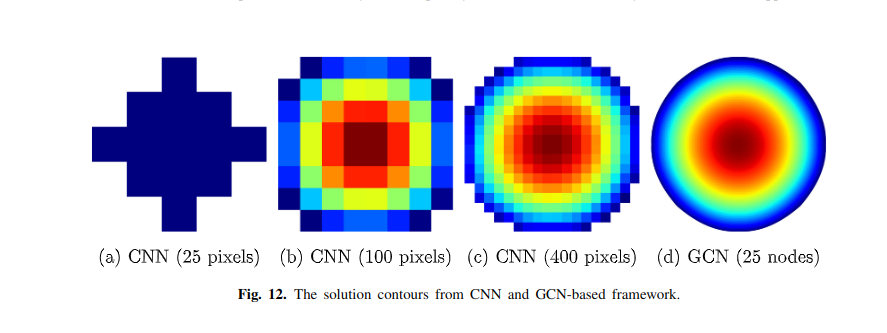
\includegraphics[width=\textwidth]{./pics/p12.png}  
\end{figure}

我们以单位圆盘为例,说明了所提出的基于 GCN 框架相对于 CNN 框架的优越性。
图12比较了不同分辨率下 CNN 和 GCN 的解轮廓。即使是一个简单的圆形,对于CNN来说都需要大量的点(见图12c)。在非结构化网格中使用相同数量的节点(25)时,基于像素的方法根本不起作用。
由于缺乏平滑的分辨场和严格的边界条件,基于 CNN 的方法效果不理想。即使分辨率$\times 8$(400像素) ,CNN 的解也不如 GCN (大约低两个数量级)精确。
此外,与基于有限体积(FV)的迭代求解器相比,GCN 由于所需的迭代次数少而显示出优势。图13进一步显示了所提出的基于 GCN 的框架在训练效率和收敛速度方面的优点。
\subsection{展望}
这项工作最重要的贡献在于算法的发展,允许直接使用 GCN 解决正向和反向偏微分方程的非结构化网格。
建议的框架是通用的,可以与各种最先进的通用网络控制器[48-52]结合使用(在pytorch上的geometric上有很多例子)。
虽然目前的工作主要集中在稳态偏微分方程,但随着进一步的发展,所提出的基于 GCN 的偏微分方程学习方法也可以扩展到求解时空偏微分方程。
例如,物理信息损失函数中的时间导数可以基于正向欧拉方案来表示,并且可以构造基于图卷积的递归网络或变压器来捕获时间依赖性[38]。

此外,该框架还可以适用于超分辨率(SR)任务,其中输入是一个有噪声的低分辨率场,输出是基于 PDE 信息的超分辨率训练。由于大多数现有的 SR 工作仍然严重依赖于 CNN,所以提出的框架有可能扩大 SR 在非结构化网格的不规则几何中的应用[53,54]。

此外,我们亦可透过 变分推断 ,将「一般通用网络」制定为一个贝叶斯网路,以处理数据噪音及量化不确定性[55]。

\section{总结}
本文提出了一种新的离散 PINN 框架,用于统一求解由偏微分方程控制的正问题和逆问题。
基于图卷积网络(GCNs)和物理信息损失函数的 Galerkin 变分公式,提出的 PINN 能够自然地处理非结构化网格的不规则域,由于多项式搜索空间减小,训练效率提高。
由于边界条件和稀疏观测数据的强制执行,该方法不需要调整惩罚参数,具有较好的鲁棒性。通过对几个线性和非线性偏微分方程正反问题的数值计算,证明了该方法的有效性。
此外,作者认为,这项工作有助于促进科学深度学习和经典数值技术的健康结合,而不是孤立彼此。


